%%%%%%%%%%%%%%%%%%%%%%%%%%%%%%%%%%%%%%%%%
% Beamer Presentation
% LaTeX Template
% Version 1.0 (10/11/12)
%
% This template has been downloaded from:
% http://www.LaTeXTemplates.com
%
% License:
% CC BY-NC-SA 3.0 (http://creativecommons.org/licenses/by-nc-sa/3.0/)
%
%%%%%%%%%%%%%%%%%%%%%%%%%%%%%%%%%%%%%%%%%

%----------------------------------------------------------------------------------------
%	PACKAGES AND THEMES
%----------------------------------------------------------------------------------------

\documentclass{beamer}

\mode<presentation> {

% The Beamer class comes with a number of default slide themes
% which change the colors and layouts of slides. Below this is a list
% of all the themes, uncomment each in turn to see what they look like.

%\usetheme{default}
%\usetheme{AnnArbor}
%\usetheme{Antibes}
%\usetheme{Bergen}
%\usetheme{Berkeley}
%\usetheme{Berlin}
%\usetheme{Boadilla}
%\usetheme{CambridgeUS}
%\usetheme{Copenhagen}
%\usetheme{Darmstadt}
%\usetheme{Dresden}
%\usetheme{Frankfurt}
%\usetheme{Goettingen}
%\usetheme{Hannover}
%\usetheme{Ilmenau}
%\usetheme{JuanLesPins}
%\usetheme{Luebeck}
\usetheme{Madrid}
%\usetheme{Malmoe}
%\usetheme{Marburg}
%\usetheme{Montpellier}
%\usetheme{PaloAlto}
%\usetheme{Pittsburgh}
%\usetheme{Rochester}
%\usetheme{Singapore}
%\usetheme{Szeged}
%\usetheme{Warsaw}

% As well as themes, the Beamer class has a number of color themes
% for any slide theme. Uncomment each of these in turn to see how it
% changes the colors of your current slide theme.

%\usecolortheme{albatross}
%\usecolortheme{beaver}
%\usecolortheme{beetle}
%\usecolortheme{crane}
%\usecolortheme{dolphin}
%\usecolortheme{dove}
%\usecolortheme{fly}
%\usecolortheme{lily}
%\usecolortheme{orchid}
%\usecolortheme{rose}
%\usecolortheme{seagull}
%\usecolortheme{seahorse}
%\usecolortheme{whale}
%\usecolortheme{wolverine}

%\setbeamertemplate{footline} % To remove the footer line in all slides uncomment this line
%\setbeamertemplate{footline}[page number] % To replace the footer line in all slides with a simple slide count uncomment this line

%\setbeamertemplate{navigation symbols}{} % To remove the navigation symbols from the bottom of all slides uncomment this line
}

\usepackage{graphicx} % Allows including images
\usepackage{booktabs}
\usepackage{stackengine}
\usepackage{amsmath}% Allows the use of \toprule, \midrule and \bottomrule in tables

%----------------------------------------------------------------------------------------
%	TITLE PAGE
%----------------------------------------------------------------------------------------

\title[Short title]{Optimization } % The short title appears at the bottom of every slide, the full title is only on the title page

\author{Siddarth kumar} % Your name

\institute[IITH] % Your institution as it will appear on the bottom of every slide, may be shorthand to save space
{
IIT Hyderabad \\ % Your institution for the title page
\medskip
\text{EE15BTECH11032} % Your email address
}
\date{\today} % Date, can be changed to a custom date

\begin{document}

\begin{frame}
\titlepage % Print the title page as the first slide
\end{frame}

\begin{frame}
\frametitle{Overview} % Table of contents slide, comment this block out to remove it
\tableofcontents % Throughout your presentation, if you choose to use \section{} and \subsection{} commands, these will automatically be printed on this slide as an overview of your presentation
\end{frame}

%----------------------------------------------------------------------------------------
%	PRESENTATION SLIDES
%----------------------------------------------------------------------------------------

%------------------------------------------------
\section{Section 4} % Sections can be created in order to organize your presentation into discrete blocks, all sections and subsections are automatically printed in the table of contents as an overview of the talk
%------------------------------------------------


\begin{frame}
\frametitle{Question 4.1}
%Express the following problem in matrix form \bigbreak
Show using \testit{e(n) = d(n) - $W^T(n)X(n)$} that \bigbreak
\nabla{\textsubscript{W(n)}e^2(n)} = \frac{\partial {e^2(n)}}{\partial W(n)} = -2X(n)d(n)+2X(n)X^T(n)W(n)
%\hspace{2cm}  \(\stackunder{min}{\textbf{x}}\) x\textsubscript{11} + x\textsubscript{12} \\


\end{frame}

%------------------------------------------------
\section{Solution}

\begin{frame}
\frametitle{Solution}
We can write e^2(n) = e(n)^T e(n)\\
using above equation,\\ 
\begin{center}{e^2(n) =  (d(n) - $W^T(n)X(n)$)^T \cdot (d(n) - $W^T(n)X(n)$)}\\
\end{center}
 As d(n) is scalar,\\

e^2(n)= d^2(n) - (X^T(n)W(n))d(n)-(W^T(n)X(n))d(n) + X^T(n)W(n)W^T(n)X(n)\\
\bigbreak
\\Differentiating w.r.t W(n) we get,
\begin{center}{
\nabla{\textsubscript{W(n)}e^2(n)} = -2X(n)d(n) + X(n)(W^T(n)X(n))\\
or \\
\end{center}
\begin{center}
\nabla{\textsubscript{W(n)}e^2(n)} = -2X(n)d(n) + X(n)(X^T(n)W(n))}
\end{center}
\end{frame}

%------------------------------------------------

\begin{frame}
\frametitle{Question 4.2}
Use the gradient descent method to obtain algorithm for solving \\

\bigbreak
\hspace{2cm}  \(\stackunder{min}{\tiny{W(n)}}\) e^2(n) \\

\end{frame}

\begin{frame}{Solution}
    From gradient descent algorithm we know \bigbreak
    W(n+1) = W(n) - \mu \cdot (\nabla{\textsubscript{W(n)}e^2(n)})
    \bigbreak
    Using $\nabla{\textsubscript{W(n)}e^2(n)}$ value from previous question we get, \bigbreak
    W(n+1) = W(n) + \mu \cdot X(n)(d(n) - X^T(n)W(n))\\
    or\\
    W(n+1) = W(n) + \mu \cdot X(n)\cdot e(n)
\end{frame}

\begin{frame}{Question 4.3}
Write a program to suppress X(n) in d(n).    
\end{frame}
\begin{frame}{Solution}
\begin{center}
    Signal with noise spectogram
\end{center}
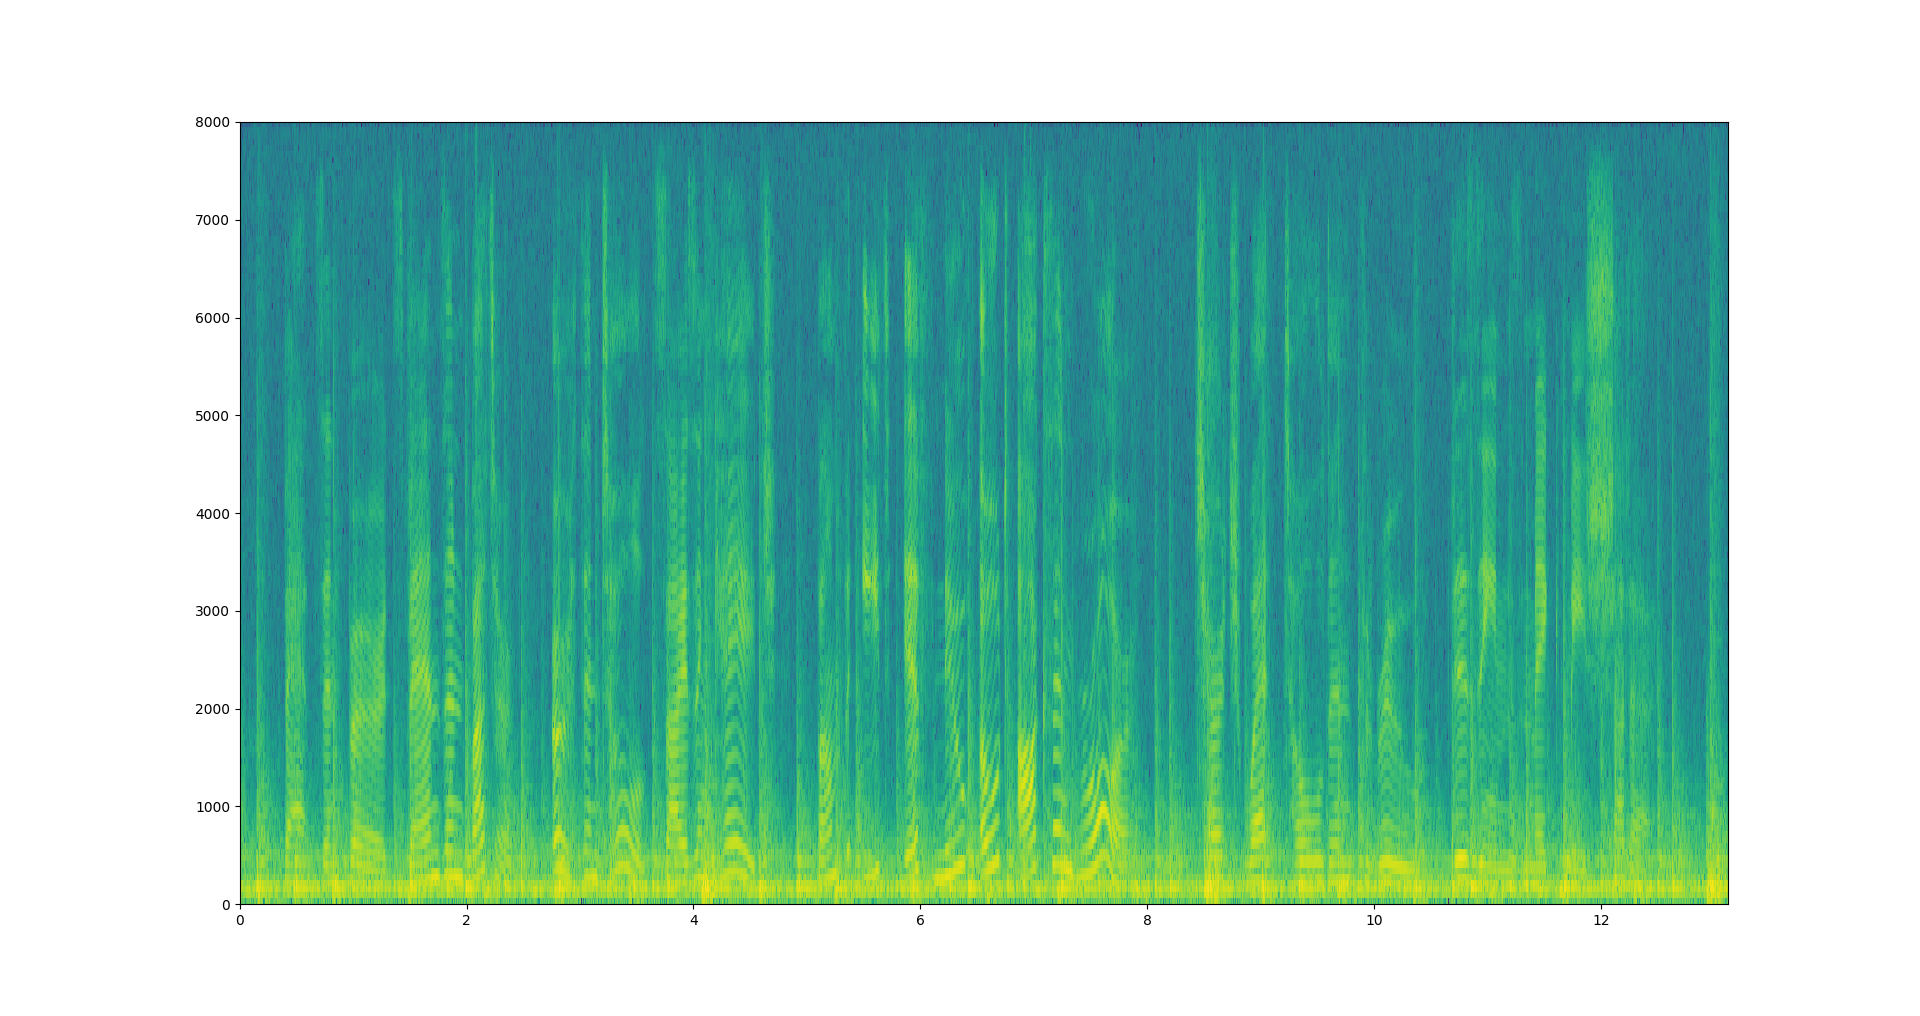
\includegraphics[scale=0.25]{signal_noise.png}
    %Code available at \url{https://pastebin.com/0Hi0hyUR}
    
\end{frame}
\begin{frame}{Solution}
\begin{center}
     Spectogram of noise
\end{center}
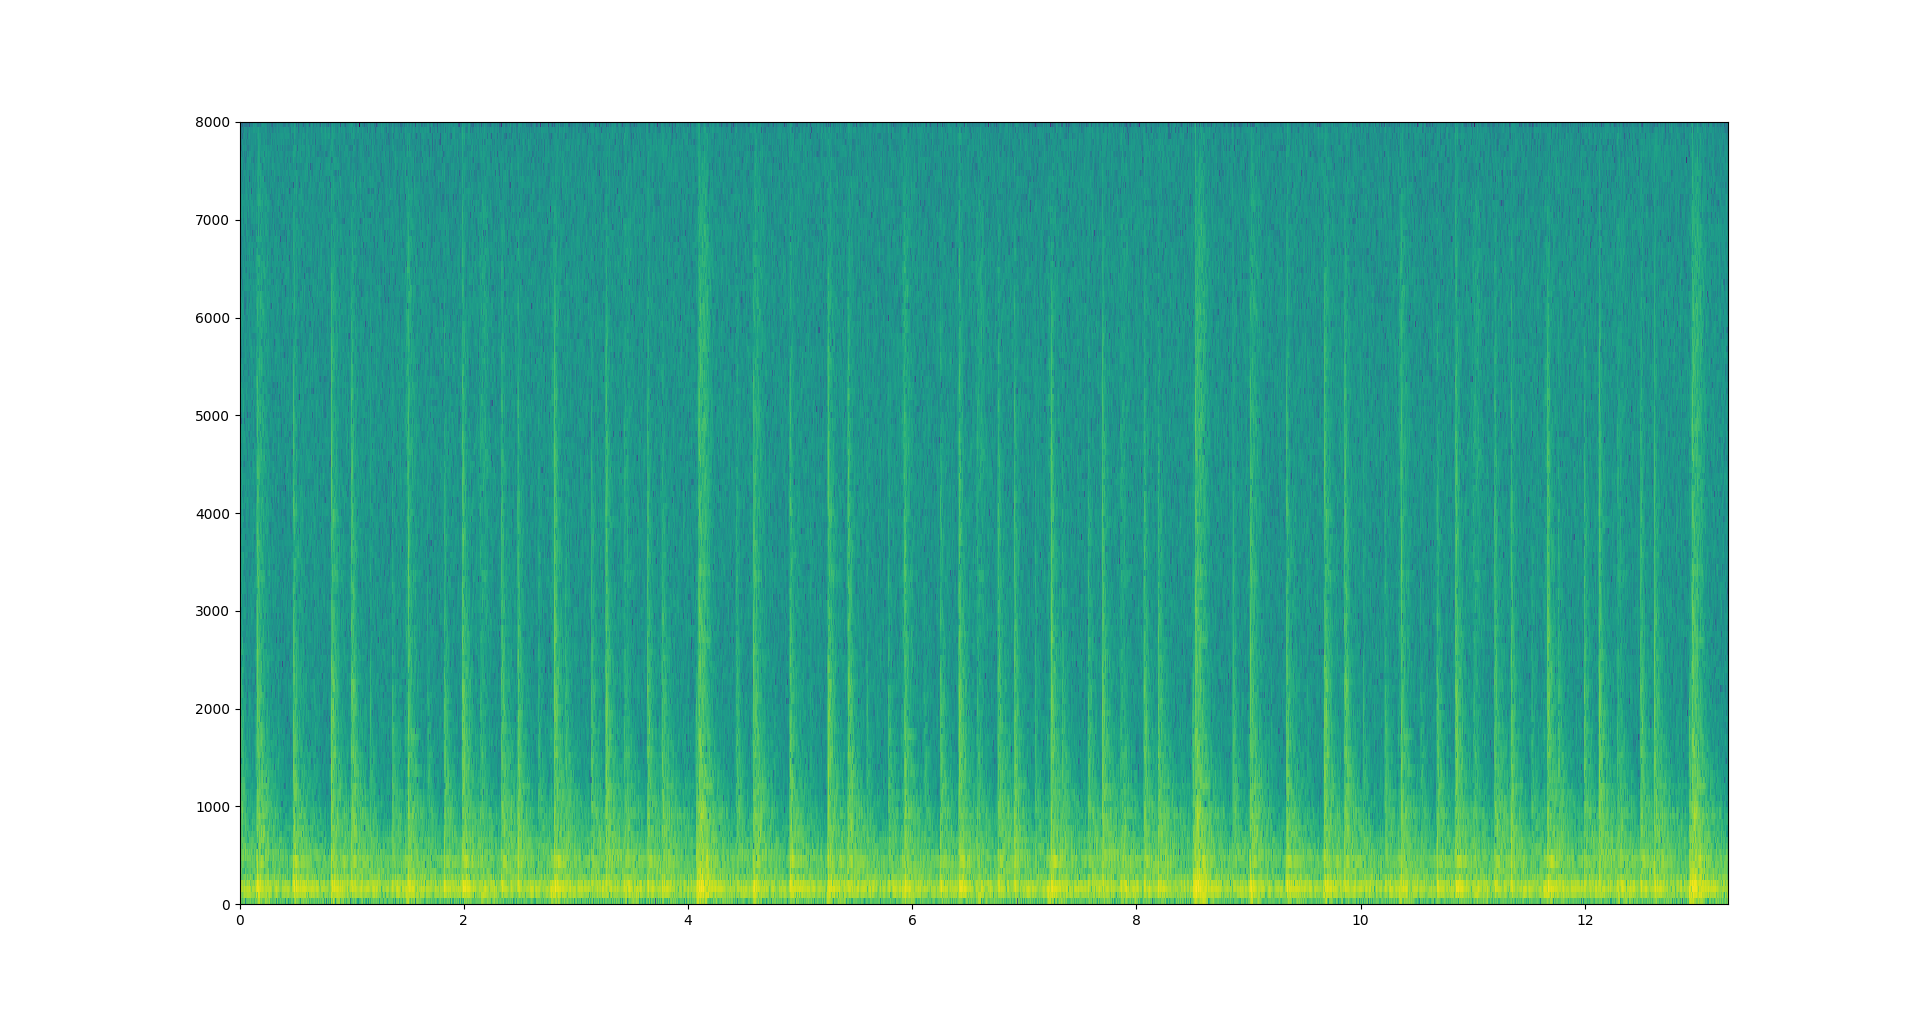
\includegraphics[scale=0.25]{noise.png}
    %Code available at \url{https://pastebin.com/0Hi0hyUR}
    
\end{frame}

\begin{frame}{Solution}
\begin{center}
    Output signal spectogram
\end{center}
\includegraphics[scale=0.23]{output1.png}
    \\ Code at \mini{\url{https://github.com/gadepall/adsp/blob/master/lms/LMS_NC_SPEECH.py}}
    
\end{frame}


\begin{frame}
\Huge{\centerline{The End}}
\end{frame}

%----------------------------------------------------------------------------------------

\end{document}